\begin{figure}[t!]
    \centering
    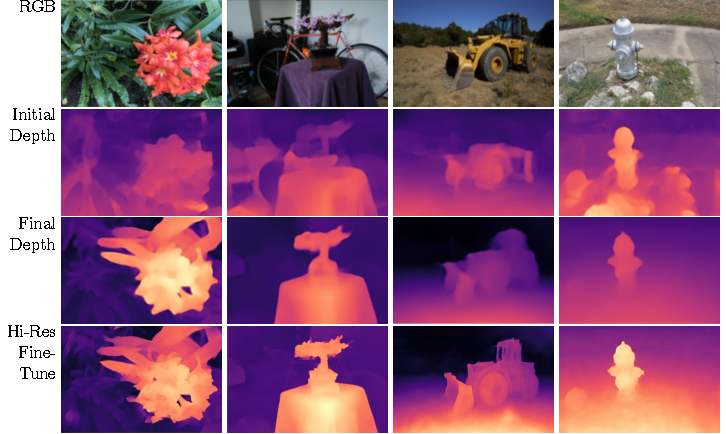
\includegraphics[width=\linewidth,]{figures/depth_vis_hires_compressed.pdf}
    \caption{\textbf{Depth Estimates Before and After Optimization.} The depth prediction neural network can either be randomly initialized or pre-trained, though pre-trained depth networks lead to much faster convergence. 
    In the second row, we show the output of the depth prediction neural network after pre-training it on a dataset consisting of CO3D, KITTI, and RealEstate10k. 
    These estimates converge to high-quality depth within only a few hundred FlowMap optimization steps. We see that the quality of the initial, pre-trained depth predictions is not critical to achieve accurate reconstructions.
    Although we estimate geometry at a lower resolution during optimization to manage memory constraints, we can quickly fine-tune at high-resolution for more detailed depth maps if necessary (bottom row). 
    }
    \label{fig:depths}
\end{figure}
